% !TEX root = ../ApproxDA-TransUNet.tex
\section{Results}
\label{sec:experiments}

We evaluate ApproxDA-TransUNet on three benchmarks spanning tasks with different spatial characteristics, comparing against DA-TransUNet and other published baselines.

\subsection{Experimental Setup}

\textbf{Datasets.} We evaluate on three representative medical image segmentation benchmarks.

\textit{Synapse Multi-Organ CT}~\cite{landman2015miccai}: 30 abdominal CT scans with an 18/12 train/test split covering 8 organ classes. Metrics: mean DSC and HD95.

\textit{Kvasir-SEG}~\cite{jha2020kvasir}: 1000 endoscopy polyp images (binary) with an 800/200 train/test split. Metrics: DSC and mIoU.

\textit{ISIC 2018}~\cite{codella2019isic}: 2594 dermoscopy skin lesion images (binary) with a 2075/519 train/test split. Metrics: DSC and mIoU.

\textbf{Implementation Details.} All experiments use an R50-ViT-B/16 backbone pretrained on ImageNet-21K, trained on NVIDIA Tesla T4 (16\,GB) GPUs. Optimizer: SGD, lr$=$0.01 with polynomial decay; batch size 24; input $224{\times}224$; 300 epochs; random rotation and flipping. Default ApproxDA-TransUNet configuration: $M{=}7$, $r{=}32$, $G{=}8$.

\textbf{Evaluation Protocol.} In accordance with established benchmark evaluation protocols for Synapse and related benchmarks~\cite{chen2021transunet,sun2024datransunet}, models are trained on the training partition and evaluated periodically (every 15 epochs) on the test split to identify peak checkpoint performance. Hyperparameter configurations ($M, r, G$, and gating mode) reported in Tables~\ref{tab:synapse}--\ref{tab:isic} correspond to the optimal settings identified in the comprehensive ablation sweeps in Section~\ref{sec:understanding}. In line with standard single-split reporting in this benchmark literature, results reflect single training runs.

\textbf{Gate Protocol.} ApproxDA-TransUNet supports four gate modes: \texttt{pam} ($\mathbf{g}{=}\mathbf{1}$, PAM only), \texttt{cam} ($\mathbf{g}{=}\mathbf{0}$, CAM only), \texttt{fixed} ($\mathbf{g}{=}0.5\cdot\mathbf{1}$, equal blend), and \texttt{learn} ($\mathbf{g}$ learned per channel). Each experiment's gate configuration is specified in the corresponding table footnote.

\subsection{Comparison with Published Methods}

Tables~\ref{tab:synapse}--\ref{tab:isic} compare ApproxDA-TransUNet against published baselines across all three benchmarks. Baseline values are compiled from published literature: for Synapse from the respective references compiled in~\cite{sun2024datransunet}, and for Kvasir-SEG and ISIC 2018 from Table~2 of DA-TransUNet~\cite{sun2024datransunet} ($256{\times}256$ input, Adam, random 75/25 split). These literature metrics provide indicative benchmarks across architectures.

\textbf{Synapse.} Table~\ref{tab:synapse} benchmarks against 11 published methods. CNN-based models plateau at 76--78\% DSC, with Att-UNet leading at 77.77\%. Transformer-based methods progressively improve: TransUNet (77.48\%), UCTransNet (78.23\%), MIM (78.59\%), Swin-Unet (79.13\%), and DA-TransUNet (79.80\%). ApproxDA-TransUNet with gate=pam, $M{=}28$, $r{=}32$ achieves \textbf{80.94\%} DSC, outperforming all compared baselines and improving by $+$1.14\% over DA-TransUNet. Its HD95 reaches 27.49\,mm (compared to 21.55\,mm for Swin-Unet and 23.48\,mm for DA-TransUNet). Section~\ref{sec:understanding} examines the underlying window-size dynamics.

\begin{table}[ht]
  \caption{Segmentation Results on Synapse Multi-Organ CT}
  \label{tab:synapse}
  \begin{center}
  \setlength{\tabcolsep}{5pt}
  \small\begin{tabular}{clcc}
    \toprule
    & Method & DSC (\%) $\uparrow$ & HD95 (mm) $\downarrow$ \\
    \midrule
    \multirow{5}{*}{\rotatebox{90}{\footnotesize CNN-based}}
      & U-Net~\cite{ronneberger2015unet}              & 76.85 & 39.70 \\
      & U-Net++~\cite{zhou2018unetpp}                 & 76.91 & 36.93 \\
      & Residual U-Net~\cite{diakogiannis2020resunet} & 76.95 & 38.44 \\
      & MultiResUNet~\cite{ibtehaz2020multiresunet}   & 77.42 & 36.84 \\
      & Att-Unet~\cite{oktay2018attention}            & 77.77 & 36.02 \\
    \midrule
    \multirow{6}{*}{\rotatebox{90}{\footnotesize Transformer-based}}
      & TransUNet~\cite{chen2021transunet}            & 77.48 & 31.69 \\
      & UCTransNet~\cite{wang2022uctransnet}          & 78.23 & 26.75 \\
      & TransNorm~\cite{azad2022transnorm}            & 78.40 & 30.25 \\
      & MIM~\cite{wang2022mim}                        & 78.59 & 26.59 \\
      & Swin-Unet~\cite{cao2022swinunet}              & 79.13 & \textbf{21.55} \\
      & DA-TransUNet~\cite{sun2024datransunet}        & \underline{79.80} & \underline{23.48} \\
    \midrule
      & \textbf{ApproxDA-TransUNet (ours)}            & \textbf{80.94} & 27.49 \\
    \bottomrule
  \end{tabular}
  \end{center}
  \vspace{-0.3em}
  \footnotesize{ApproxDA: gate=pam, $M{=}28$, $r{=}32$, $G{=}8$.}
\end{table}

\textbf{Kvasir-SEG.} On polyp segmentation (Table~\ref{tab:kvasir}), U-Net leads the CNN-based group (88.22\% DSC) while TransUNet (87.91\%) and DA-TransUNet$^\dag$ (88.44\%) are the strongest Transformer-based entries. ApproxDA-TransUNet with gate=pam, $M{=}56$ achieves \textbf{90.17\%} DSC and \textbf{84.27\%} mIoU, attaining top performance with a $+$1.73\% DSC improvement over matched re-run DA-TransUNet and lower boundary distance (44.35 vs.\ 53.04 pixels). HD95 on Kvasir-SEG is reported in pixels due to lack of physical spacing calibration.

\begin{table}[ht]
  \caption{Segmentation Results on Kvasir-SEG Polyp}
  \label{tab:kvasir}
  \begin{center}
  \setlength{\tabcolsep}{3pt}
  \begin{tabular}{lccc}
    \toprule
    Method & DSC (\%) $\uparrow$ & mIoU (\%) $\uparrow$ & HD95 (px) $\downarrow$ \\
    \midrule
    U-Net~\cite{ronneberger2015unet}           & 88.22 & 80.12 & -- \\
    Att-Unet~\cite{oktay2018attention}         & 86.61 & 78.01 & -- \\
    U-Net++~\cite{zhou2018unetpp}              & 86.57 & 77.67 & -- \\
    Res-UNet~\cite{diakogiannis2020resunet}    & 77.85 & 66.04 & -- \\
    TransUNet~\cite{chen2021transunet}         & 87.91 & 80.03 & -- \\
    DA-TransUNet~\cite{sun2024datransunet}$^\dag$ & \underline{88.44} & \underline{81.70} & \underline{53.04} \\
    \midrule
    \textbf{ApproxDA-TransUNet (ours)}         & \textbf{90.17} & \textbf{84.27} & \textbf{44.35} \\
    \bottomrule
  \end{tabular}
  \end{center}
  \vspace{-0.3em}
  \footnotesize{$^\dag$DA-TransUNet re-run with our training settings and split (DSC 88.44\%, vs.\ 88.47\% reported in~\cite{sun2024datransunet}); all other rows are literature values from~\cite{sun2024datransunet}. ApproxDA: gate=pam, $M{=}56$, $r{=}32$.}
\end{table}

\textbf{ISIC 2018.} On skin lesion segmentation (Table~\ref{tab:isic}), CNN-based methods cluster between 83--88\% DSC, with TransUNet (88.78\%) and DA-TransUNet (88.88\%) leading among Transformer-based approaches. ApproxDA-TransUNet with gate=learn, $M{=}7$ achieves \textbf{89.58\%} DSC ($+$0.70\% over reported DA-TransUNet), while mIoU (82.66\%) is comparable to DA-TransUNet (82.78\%). Baseline values are referenced from~\cite{sun2024datransunet}. The minimal performance spread across window sizes on this dataset is detailed in Section~\ref{sec:obs2}.

\begin{table}[ht]
  \caption{Segmentation Results on ISIC 2018 Skin Lesion}
  \label{tab:isic}
  \begin{center}
  \renewcommand{\arraystretch}{1.15}
  \setlength{\tabcolsep}{6pt}
  \begin{tabular}{lcc}
    \toprule
    Method & DSC (\%) $\uparrow$ & mIoU (\%) $\uparrow$ \\
    \midrule
    U-Net~\cite{ronneberger2015unet}           & 87.22 & 81.14 \\
    Att-Unet~\cite{oktay2018attention}         & 87.60 & 81.51 \\
    U-Net++~\cite{zhou2018unetpp}              & 87.30 & 81.33 \\
    Res-UNet~\cite{diakogiannis2020resunet}    & 83.32 & 76.51 \\
    TransUNet~\cite{chen2021transunet}         & 88.78 & 82.63 \\
    DA-TransUNet~\cite{sun2024datransunet}     & \underline{88.88} & \textbf{82.78} \\
    \midrule
    \textbf{ApproxDA-TransUNet (ours)}         & \textbf{89.58} & \underline{82.66} \\
    \bottomrule
  \end{tabular}
  \end{center}
  \vspace{-0.3em}
  \footnotesize{Baseline values from Table~2 of~\cite{sun2024datransunet}. ApproxDA: gate=learn, $M{=}7$, $r{=}32$, $G{=}8$.}
\end{table}

Overall, ApproxDA-TransUNet demonstrates consistently high DSC across all three benchmarks (Figure~\ref{fig:qualitative} illustrates qualitative segmentations), while showing that performance sensitivity to window scale is strongly task-dependent.

\begin{figure}[b]
  \centering
  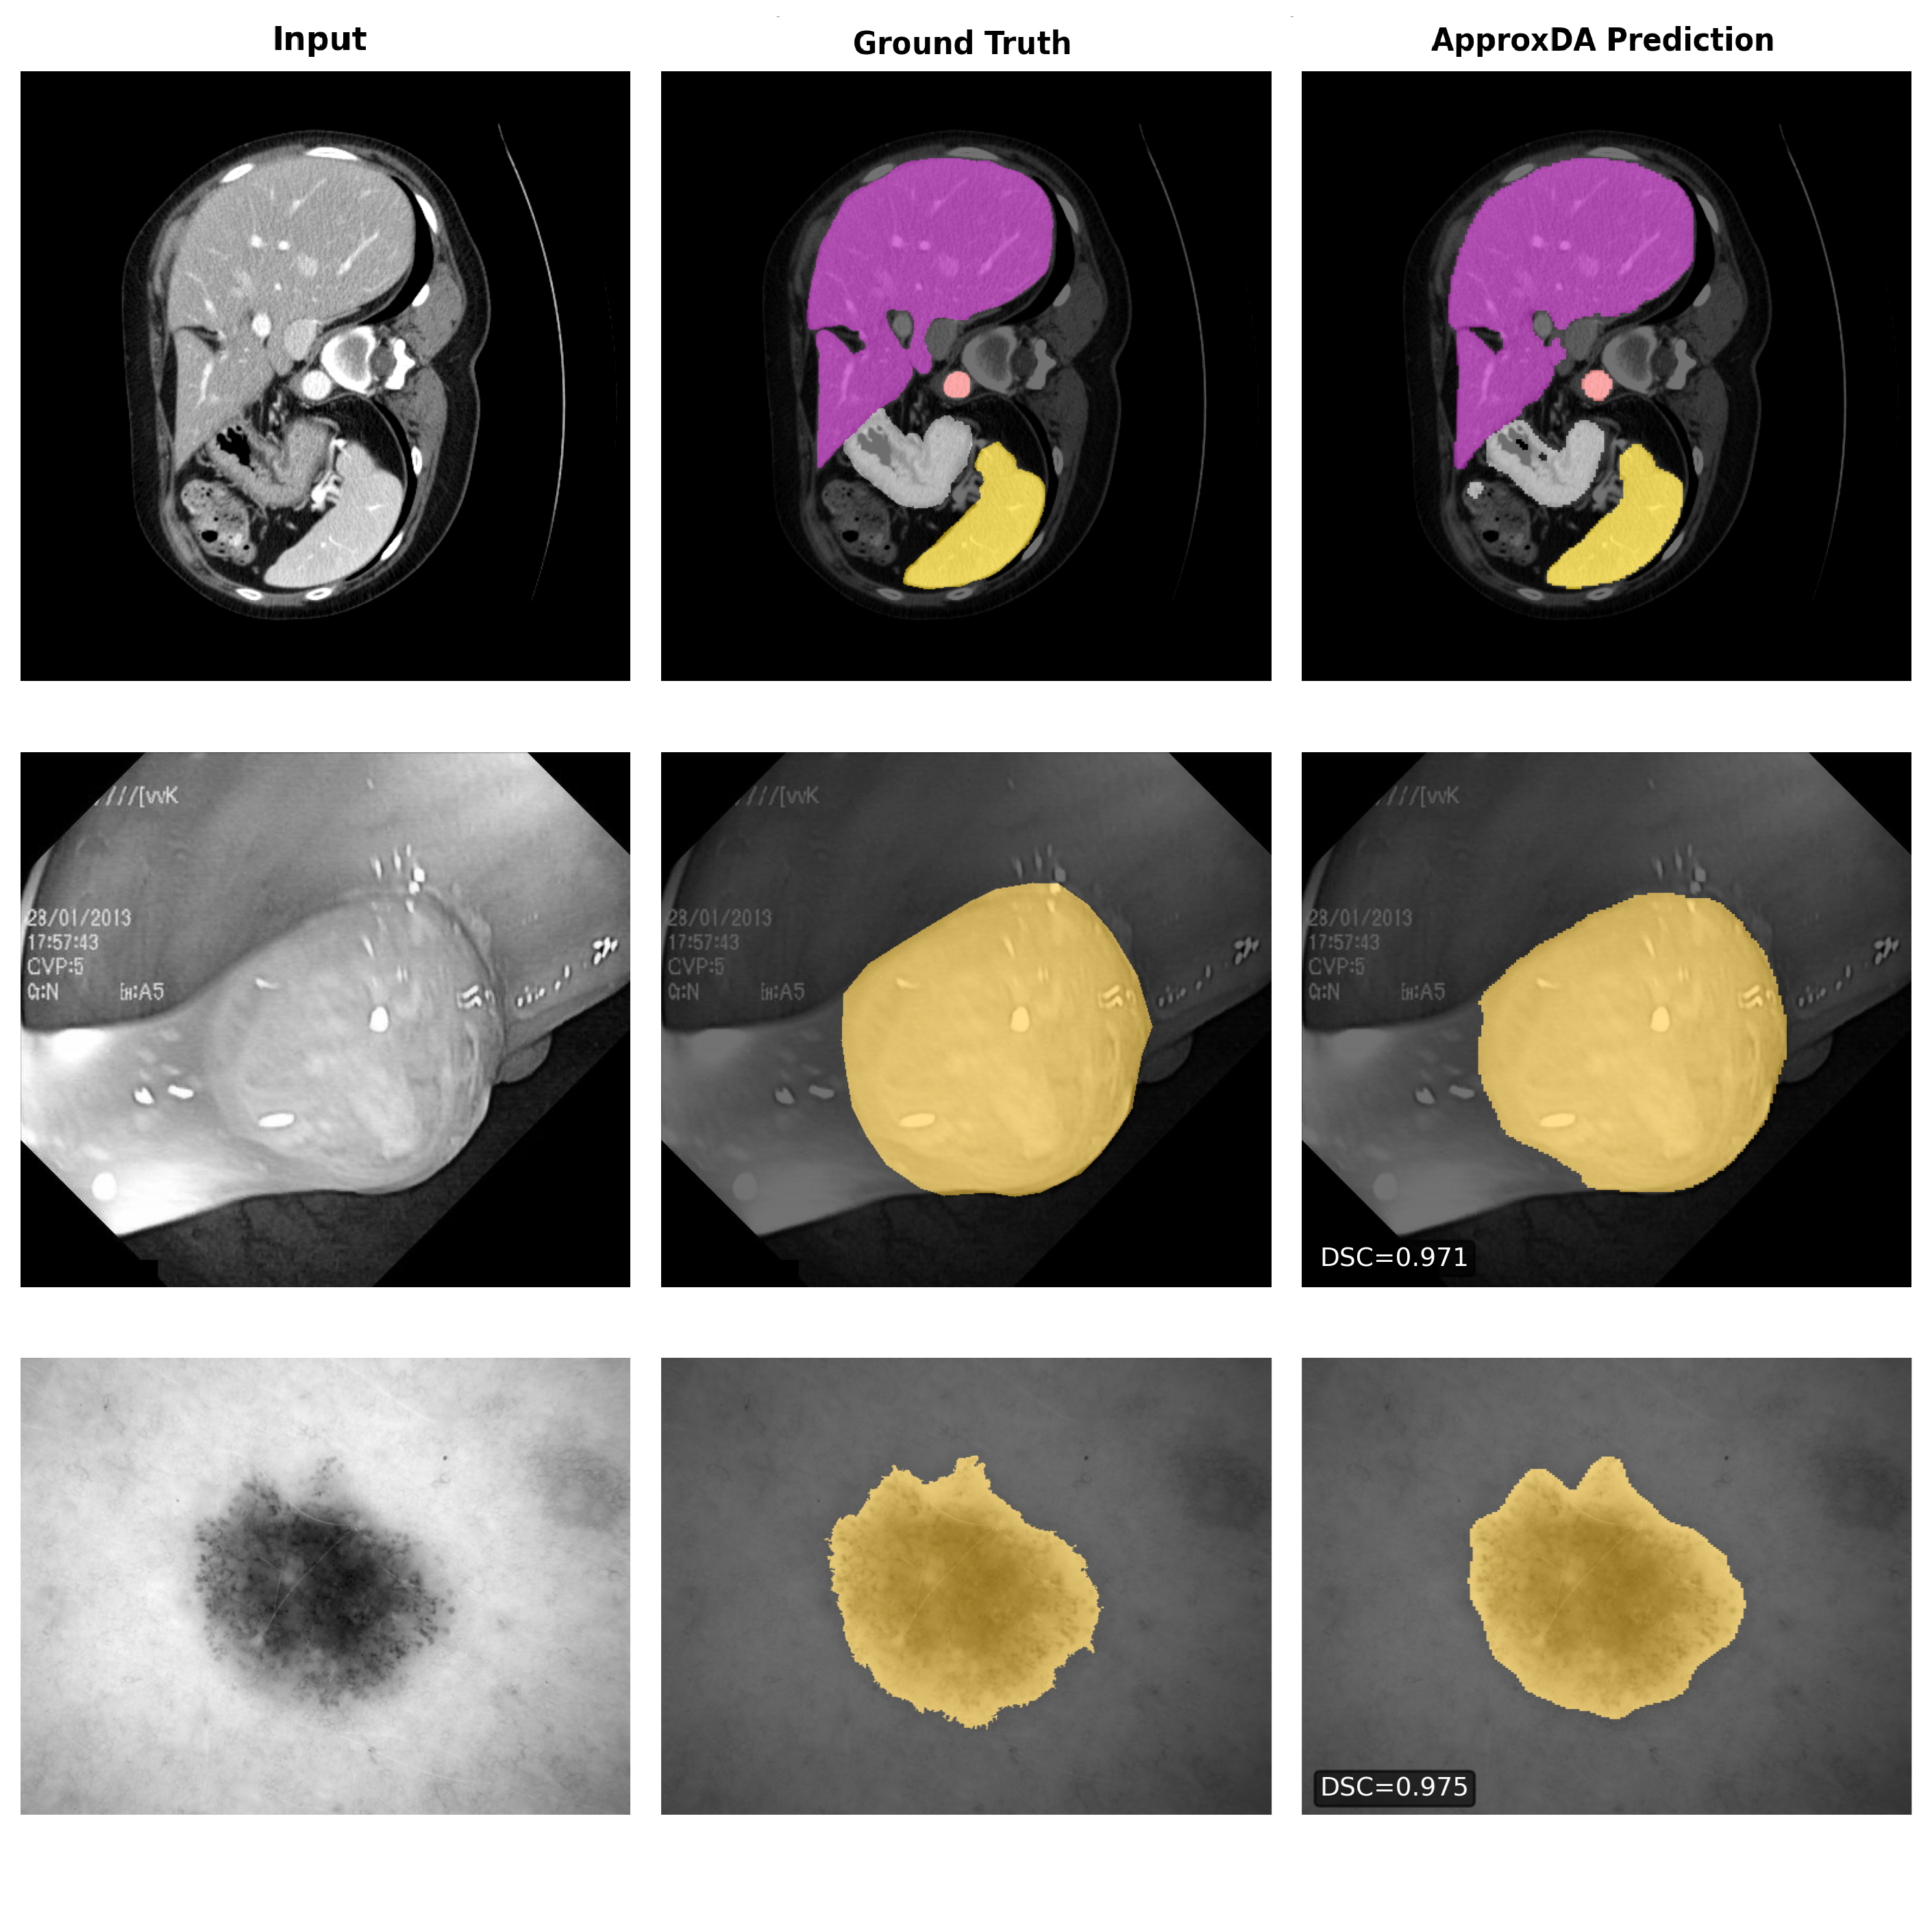
\includegraphics[width=\columnwidth]{figures/fig_qualitative_cross_task.png}
  \caption{Qualitative segmentation comparison (columns: input, ground truth, DA-TransUNet, ApproxDA). \textbf{Top (Synapse, $M{=}28$):} multi-organ CT; ApproxDA 80.94\% DSC ($+$1.14\%). \textbf{Middle (Kvasir-SEG, $M{=}56$):} polyp; 90.17\% DSC ($+$1.73\%). \textbf{Bottom (ISIC 2018, $M{=}7$):} skin lesion; 89.58\% DSC ($+$0.70\%). Gains are relative to the DA-TransUNet values in Tables~\ref{tab:synapse}--\ref{tab:isic}.}
  \label{fig:qualitative}
\end{figure}

\subsection{Computational Cost and Parameter Profile}
\label{sec:efficiency}

Table~\ref{tab:efficiency} reports parameter counts and FLOPs evaluated with a standardized profiling tool across all architectures. While spatial windowing and low-rank projection reduce the asymptotic complexity of the core affinity matrix (Section~\ref{sec:method}), total computational cost is primarily determined by the hybrid CNN--ViT backbone ($\sim$85M parameters). Furthermore, by preserving full channel dimensions $C$ (omitting the $C/16$ bottleneck compression) and placing an additional attention block at the fine $112{\times}112$ skip resolution, ApproxDABlocks emphasize representation fidelity. ApproxDA-TransUNet is thus conceived as a controlled diagnostic vehicle for probing context dynamics and approximation mechanisms rather than a specialized low-latency edge architecture.

\begin{table}[ht]
  \caption{Parameters and FLOPs (fvcore, one $224{\times}224$ slice)}
  \label{tab:efficiency}
  \begin{center}
  \setlength{\tabcolsep}{3pt}
  \begin{tabular}{lccc}
    \toprule
    Method & Params (M) & GFLOPs & Attn.\ GFLOPs \\
    \midrule
    DA-TransUNet~\cite{sun2024datransunet}  & 106.56 & 30.2 & 0.87 \\
    ApproxDA (gate=pam, $M$=7)              & 108.98 & 32.1 & 2.73 \\
    ApproxDA (gate=learn, $M$=7)            & 109.90 & 32.1 & 2.74 \\
    \bottomrule
  \end{tabular}
  \end{center}
  \vspace{-0.3em}
  \footnotesize{One multiply--add is counted as one FLOP. Parameter counts and FLOPs reflect active forward-pass modules at $224{\times}224$ input resolution (three attention blocks in DA-TransUNet, four in ApproxDA-TransUNet).}
\end{table}
